% ============================================================
% When Does Search Beat Reasoning?
% A Topology-Driven Diagnostic of A* versus Chain-of-Thought
% ============================================================
% Format: Single-column, 11pt
% Compatible with Overleaf — upload this folder directly

\documentclass[11pt]{article}

% ── Must come BEFORE tikz/pgfplots load xcolor internally ──
\PassOptionsToPackage{dvipsnames}{xcolor}

% ── Core Packages ──
\usepackage[utf8]{inputenc}
\usepackage[T1]{fontenc}
\usepackage{times}
\usepackage[margin=2.5cm]{geometry}
\usepackage{microtype}
\usepackage{setspace}
\onehalfspacing

% ── Math ──
\usepackage{amsmath,amssymb,amsthm}

% ── Tables & Figures ──
\usepackage{booktabs}
\usepackage{multirow}
\usepackage{tabularx}
\usepackage{array}
\usepackage{graphicx}
\usepackage{float}
\usepackage{caption}
\usepackage{subcaption}

% ── Plots ──
\usepackage{tikz}
\usepackage{pgfplots}
\pgfplotsset{compat=1.17}

% ── Colors & Links ──
\usepackage[dvipsnames]{xcolor}
\usepackage[colorlinks=true,linkcolor=MidnightBlue,citecolor=OliveGreen,urlcolor=BrickRed]{hyperref}

% ── Bibliography ──
\usepackage[numbers,sort&compress]{natbib}

% ── Misc ──
\usepackage{enumitem}
\usepackage{tcolorbox}

% ── Theorem environments ──
\newtheorem{theorem}{Theorem}
\newtheorem{definition}[theorem]{Definition}
\newtheorem{proposition}[theorem]{Proposition}

% ── Custom commands ──
\newcommand{\astar}{A$^*$\xspace}
\newcommand{\cmark}{\textcolor{OliveGreen}{\ding{51}}}
\newcommand{\xmark}{\textcolor{BrickRed}{\ding{55}}}
\newcommand{\pp}{\,pp}
\newcommand{\ie}{\emph{i.e.},\xspace}
\newcommand{\eg}{\emph{e.g.},\xspace}
\newcommand{\cf}{\emph{cf.}\xspace}
\newcommand{\etal}{\emph{et al.}\xspace}

% ── Suppress xspace warning ──
\usepackage{xspace}

% ── Header ──
\usepackage{fancyhdr}
\pagestyle{fancy}
\fancyhf{}
\fancyhead[L]{\small\textit{When Does Search Beat Reasoning?}}
\fancyhead[R]{\small\thepage}
\renewcommand{\headrulewidth}{0.4pt}

% ============================================================
\begin{document}

% ── Title Block ──
\begin{center}
{\LARGE\bfseries When Does Search Beat Reasoning?\\[4pt]
A Topology-Driven Diagnostic of A* versus Chain-of-Thought}\\[1.5em]
{\large [Author Names]\textsuperscript{1}}\\[0.3em]
{\normalsize \textsuperscript{1}[Affiliation]}\\[0.3em]
{\small\texttt{[email@institution.edu]}}\\[1.5em]
\end{center}

% ── Abstract ──
\begin{abstract}
Chain-of-Thought (CoT) prompting and tree-search methods have independently advanced LLM reasoning, yet no systematic study explains \emph{when} search-based reasoning outperforms linear reasoning or vice versa. We treat A* search as a \textbf{unified search framework}---subsuming breadth-first, depth-first, and best-first strategies under a single admissible heuristic---and conduct a controlled comparison against CoT on 2,151 questions across three benchmarks (LogicQA, StrategyQA, HotpotQA) using LLaMA~3.1-8B. Aggregate results are equivocal: A* leads on StrategyQA (+10.3\pp) and HotpotQA (+3.3\pp) but trails on LogicQA ($-$0.9\pp). To resolve this ambiguity, we introduce two complementary diagnostic lenses. First, a \textbf{Reasoning Topology Framework} characterises each question by 13~structural features and clusters problems into four topology types, showing that branching complexity---not dataset identity---predicts strategy success. Second, \textbf{cross-dataset topic modelling} (NMF, 8~categories) reveals that A* dominates in 5~categories covering \textbf{81.4\%} of the corpus---all requiring multi-hop evidence chaining---while CoT wins on the remaining 18.6\% of single-step inference tasks. A topology-aware router that sees \emph{zero model outputs} recovers 26.1\% of the oracle gap, outperforming all output-based routers and confirming that the bottleneck is recognising problem structure, not evaluating trace quality. We further document the Fluency--Correctness Asymmetry (38\% of divergent cases), a failure-mode taxonomy (91.1\% overthinking), and a $3.5\times$ search-as-capability-amplification effect for small language models. Together, these findings establish that neither strategy universally dominates: the right choice is determined by the reasoning topology of the problem.
\end{abstract}

\vspace{0.5em}
\noindent\textbf{Keywords:} A* search, chain-of-thought, LLM reasoning, topic modelling, reasoning topology, adaptive routing

% ============================================================
\section{Introduction}
\label{sec:intro}

The emergence of Chain-of-Thought (CoT) prompting~\citep{wei2022chain} demonstrated that large language models reason more reliably when they externalise intermediate steps. Subsequent work extended this insight from linear chains to richer structures: Tree-of-Thoughts (ToT;~\citealt{yao2024tree}) explores alternative reasoning paths via breadth-first or depth-first search, Graph-of-Thoughts (GoT;~\citealt{besta2024graph}) permits arbitrary reasoning topologies, and MCTS-based approaches~\citep{hao2023reasoning} apply Monte Carlo rollouts to reasoning trees. These advances raise a fundamental question that remains unanswered:

\begin{quote}
\emph{When does structured search actually improve over linear reasoning, and when does it hurt?}
\end{quote}

Prior comparisons treat search-based and linear reasoning as competing paradigms, reporting aggregate accuracy on individual benchmarks. But aggregates conceal systematic structure. A method that wins by 10 points on commonsense reasoning and loses by 1 point on formal logic looks equivalent on average---yet behaves very differently at the instance level.

\paragraph{Why A* as a unified framework.}
Rather than testing breadth-first, depth-first, best-first, and beam search separately, we adopt A* search as the \textbf{generalisation}: by varying the heuristic function, A* reduces to each of these strategies. When the heuristic $h(n)$ is admissible---never overestimating the cost to goal---A* guarantees optimality~\citep{hart1968formal}. This lets us study the value of \emph{guided search itself} rather than the idiosyncrasies of any particular search variant. Our A* formulation uses an LLM-generated heuristic that scores partial reasoning states by their estimated proximity to a correct answer, with a critic model providing the evaluation signal.

\paragraph{The inconsistency problem.}
We evaluate A* and CoT on 2,151 questions across three benchmarks using LLaMA~3.1-8B, and find that aggregate results are \textbf{inconsistent}: A* leads on StrategyQA (+10.3\pp) and HotpotQA (+3.3\pp) but trails on LogicQA ($-$0.9\pp). Self-consistency~\citep{wang2023self} and Tree-of-Thoughts fall between the two. No single strategy dominates, and the aggregate numbers provide no actionable guidance for deployment.

\paragraph{Our approach.}
Rather than declaring a winner, we ask \emph{why} the methods diverge. We bring two diagnostic tools to bear:

\begin{enumerate}[leftmargin=1.5em,itemsep=2pt]
\item \textbf{Reasoning Topology Framework}---A set of 13~structural features (question length, context complexity, branching coefficient, logical connectives, hop count) that characterise each problem's reasoning structure. K-means clustering on these features yields 4~topology types with distinct strategy preferences (\S\ref{sec:topology}).
\item \textbf{Cross-dataset Topic Modelling}---Non-negative Matrix Factorisation (NMF) on 2,151 question texts identifies 8~content categories that cut across datasets. By measuring A* versus CoT accuracy within each category on \emph{fully balanced} data (2,151~$\times$~2), we determine that A* dominates in 5~categories covering 81.4\% of the corpus (\S\ref{sec:topic}).
\end{enumerate}

These two lenses converge on a single structural explanation: \textbf{A* wins whenever the correct answer requires traversing a chain of two or more interdependent facts, where greedy commitment at hop~1 propagates errors to the final answer.} When only one inference step separates question from answer, CoT's linear approach is sufficient and A*'s branching adds overhead without benefit.

\paragraph{Contributions.}
\begin{enumerate}[leftmargin=1.5em,itemsep=2pt]
\item A formal admissibility analysis for LLM-based A* search with three constructive cases and empirical validation (\S\ref{sec:admissibility}).
\item A Reasoning Topology Framework with 4~empirically validated cluster types (\S\ref{sec:topology}).
\item The finding that A* dominates in 81.4\% of question categories via cross-dataset topic modelling (\S\ref{sec:topic}).
\item A topology-aware pre-generation router that outperforms all output-based routers (\S\ref{sec:routing}).
\item The Fluency--Correctness Asymmetry quantified at 38.0\% (\S\ref{sec:fluency}).
\item A failure-mode taxonomy showing 91.1\% of A* failures are overthinking (\S\ref{sec:failure}).
\item Evidence that A* amplifies small language models by $3.5\times$ on multi-hop tasks (\S\ref{sec:slm}).
\end{enumerate}

% ============================================================
\section{Methodology}
\label{sec:method}

\subsection{A* Search for LLM Reasoning}
\label{sec:astar_method}

We formalise reasoning as a graph search problem. Each node $n$ represents a partial reasoning state (the set of intermediate conclusions reached so far). Edges correspond to single reasoning steps generated by the LLM. A* maintains an open list of nodes sorted by $f(n) = g(n) + h(n)$, where $g(n)$ is the accumulated cost (tokens consumed) and $h(n)$ is the heuristic estimate of remaining cost to a correct answer.

\paragraph{State representation.}
A state $s$ is a tuple $(\mathbf{q}, \mathbf{c}, \mathcal{P})$ where $\mathbf{q}$ is the question, $\mathbf{c}$ is the context, and $\mathcal{P} = \{p_1, \ldots, p_k\}$ is the set of premises derived so far.

\paragraph{Expansion.}
At each step, A* pops the most promising node and generates $N_c$ candidate successors by prompting the LLM to extend the reasoning by one step, each using a different inference angle (\eg supporting evidence, counterargument, factual lookup). We use $N_c = 3$ throughout.

\paragraph{Heuristic evaluation.}
A critic model (DeepSeek-R1-Distill-Qwen-14B) scores each successor for (a)~factual consistency with the context and (b)~estimated reasoning completeness. The critic returns a score in $[0, 1]$ converted to $h(n) = 1 - \text{score}$, so higher-quality states have lower estimated remaining cost.

\paragraph{Termination.}
Search terminates when a node's reasoning chain reaches a definitive answer, or when a budget of $B = 15$ expansions is exhausted. The highest-scoring terminal node's answer is returned.

\subsection{Admissibility of the LLM Heuristic}
\label{sec:admissibility}

A heuristic $h(n)$ is admissible if $h(n) \leq h^*(n)$ for all nodes~$n$, where $h^*(n)$ is the true remaining cost. In classical planning, admissibility ensures A* finds the optimal solution. We identify three sufficient conditions under which the LLM-generated heuristic approximates admissibility:

\begin{proposition}[Sufficient Conditions for Heuristic Admissibility]
\label{prop:admissibility}
Let $h(n) = 1 - \mathrm{score}(n)$ be the critic-generated heuristic. Then $h(n)$ approximates admissibility under any of:
\begin{enumerate}[label=\textbf{Case \arabic*},leftmargin=3em,itemsep=4pt]
\item \textbf{(Monotone scoring).} If the critic assigns monotonically increasing scores to states with strictly more correct premises, then $h(n)$ never overestimates, since adding correct premises can only reduce remaining work. This gives exact admissibility.
\item \textbf{(Conservative estimation).} If $\mathbb{E}[\mathrm{score}(n)] \leq \mathrm{score}^*(n)$ (systematic underestimation), then $\mathbb{E}[h(n)] \geq h^*(n)$, making the heuristic admissible \emph{in expectation}. This weaker guarantee implies that A* finds the optimal solution with high probability over repeated runs but does not guarantee optimality on every single run.
\item \textbf{(Bounded overestimation).} If $|\mathrm{score}(n) - \mathrm{score}^*(n)| \leq \epsilon$, then A* finds a solution within $\epsilon$ of optimal ($\epsilon$-admissibility), guaranteeing bounded sub-optimality~\citep{hart1968formal}.
\end{enumerate}
\end{proposition}

\paragraph{Empirical validation.}
We measure the critic's behaviour on 500~annotated reasoning states (100 per dataset for StrategyQA and HotpotQA, 300 for LogicQA). The DeepSeek critic underestimates the ground-truth reasoning progress (mean score $= 0.43$ vs.\ human-assessed progress $= 0.58$; paired $t$-test $p < 0.001$), satisfying Case~2. The overestimation rate is 12.3\% of nodes, with maximum overestimation $\epsilon_\text{max} = 0.14$, providing an empirical bound for Case~3. We note that these conditions are \emph{sufficient but not necessary}---A* can still be effective even when the heuristic is occasionally inadmissible, as the search budget acts as a regulariser.

\subsection{Comparison Methods}
\label{sec:baselines}

We compare five reasoning strategies, all using LLaMA~3.1-8B as the reasoning model via Ollama:

\begin{itemize}[leftmargin=1.5em,itemsep=2pt]
\item \textbf{CoT}: Zero-shot chain-of-thought with ``Let's think step by step''~\citep{wei2022chain}.
\item \textbf{Self-Consistency (SC)}: Majority vote over 5~sampled CoT traces~\citep{wang2023self}.
\item \textbf{Tree-of-Thoughts (ToT)}: BFS over 3~candidates per step, 5-step depth~\citep{yao2024tree}.
\item \textbf{A* Search}: As described above.
\item \textbf{Oracle}: Per-instance best of A* and CoT (upper bound).
\end{itemize}

\subsection{Benchmarks and Data}
\label{sec:data}

We evaluate on three benchmarks spanning different reasoning demands:

\begin{itemize}[leftmargin=1.5em,itemsep=2pt]
\item \textbf{LogicQA}~\citep{liu2020logiqa}: 651~formal logic questions (4-way multiple choice).
\item \textbf{StrategyQA}~\citep{geva2021did}: 500~commonsense questions requiring implicit multi-step reasoning (yes/no).
\item \textbf{HotpotQA}~\citep{yang2018hotpotqa}: 1,000~multi-hop factual questions (free-form answer).
\end{itemize}

\paragraph{Fair comparison protocol.}
We run both A* and CoT on \emph{exactly the same questions} with \emph{exactly the same model}. Prior work (including our own earlier results) compared A* with LLaMA~3.1-8B against CoT with Qwen-0.5B---a confound that conflated the $16\times$ parameter gap with the reasoning strategy difference. We explicitly filled all CoT gaps to produce a fully balanced $2{,}151 \times 2$ comparison.

\paragraph{Generation parameters.}
All experiments use Ollama~v0.5 with temperature $\tau = 0.7$, top-$p = 0.9$, and maximum generation length of 512~tokens per reasoning step. For self-consistency, we sample 5~traces with $\tau = 0.9$ to encourage diversity. For Tree-of-Thoughts, we use BFS with 3~candidates per step and 5-step depth. A* uses $N_c = 3$ candidate expansions per node and a budget of $B = 15$ total expansions. All random seeds are fixed at 42. The critic model (DeepSeek-R1-Distill-Qwen-14B) uses $\tau = 0.3$ for more deterministic scoring. Exact prompt templates are provided in Appendix~\ref{app:prompts}.

\subsection{Reasoning Topology Features}
\label{sec:features}

We define 13~structural features for each question, computed without running any model (\ie pre-generation). These features enable routing decisions before inference begins. The full feature set is described in Table~\ref{tab:features}.

\begin{table}[t]
\centering
\caption{Reasoning topology features. All features are computed from the raw question and context text without any LLM inference.}
\label{tab:features}
\small
\begin{tabular}{@{}llp{6cm}@{}}
\toprule
\textbf{Feature} & \textbf{Symbol} & \textbf{Description} \\
\midrule
Question length & $q_\text{len}$ & Token count of question \\
Context length & $c_\text{len}$ & Token count of full context \\
Context sentences & $c_\text{sent}$ & Number of sentences \\
Logical connectives & $\mathrm{conn}$ & Count of \emph{if, then, therefore, because, unless} \\
Negation markers & $\mathrm{neg}$ & Count of \emph{not, no, never, neither} \\
Comparatives & $\mathrm{cmp}$ & Count of \emph{more, less, better, worse, than} \\
Question marks & $q_?$ & Number of question marks \\
Hop count & $\mathrm{hop}$ & Estimated reasoning hops (dep.\ parse) \\
Contextual density & $\mathrm{con}$ & Entities per sentence in context \\
Distractors & $\mathrm{dest}$ & Number of candidate options (MCQ) \\
Branching coefficient & $\mathrm{bc}$ & $c_\text{sent} \times \mathrm{hop} \;/\; q_\text{len}$ \\
Reasoning depth & $\ell$ & Max.\ dependency parse depth \\
Number of options & $n_\text{opt}$ & Answer options available \\
\bottomrule
\end{tabular}
\end{table}

% ============================================================
\section{Results}
\label{sec:results}

\subsection{Aggregate Performance: The Inconsistency}
\label{sec:aggregate}

Table~\ref{tab:aggregate} presents the aggregate results. The headline finding is \textbf{inconsistency}: no strategy uniformly dominates.

\begin{table}[t]
\centering
\caption{Aggregate accuracy (\%) across three benchmarks with 95\% Wilson confidence intervals. Best per dataset in \textbf{bold}. Oracle = per-instance best of A* and CoT. $^\dagger$McNemar's test (A* vs.\ CoT): $p < 0.001$ on StrategyQA, $p = 0.61$ on LogicQA, $p = 0.048$ on HotpotQA.}
\label{tab:aggregate}
\small
\begin{tabular}{@{}lccc@{}}
\toprule
\textbf{Method} & \textbf{StrategyQA} ($n{=}500$) & \textbf{LogicQA} ($n{=}651$) & \textbf{HotpotQA} ($n{=}1000$) \\
\midrule
CoT & 64.52 {\scriptsize$\pm$4.2} & \textbf{45.78} {\scriptsize$\pm$3.8} & 76.80 {\scriptsize$\pm$2.6} \\
Self-Consistency & 71.22 {\scriptsize$\pm$4.0} & 46.10 {\scriptsize$\pm$3.8} & 78.21 {\scriptsize$\pm$2.6} \\
Tree-of-Thoughts & 72.24 {\scriptsize$\pm$3.9} & 46.21 {\scriptsize$\pm$3.8} & 78.45 {\scriptsize$\pm$2.5} \\
\textbf{A* Search}$^\dagger$ & \textbf{74.80} {\scriptsize$\pm$3.8} & 44.85 {\scriptsize$\pm$3.8} & \textbf{80.10} {\scriptsize$\pm$2.5} \\
\midrule
Oracle (A*$\cup$CoT) & 84.59 {\scriptsize$\pm$3.2} & 59.29 {\scriptsize$\pm$3.8} & 94.20 {\scriptsize$\pm$1.4} \\
\bottomrule
\end{tabular}
\end{table}

A* leads on StrategyQA (+10.3\pp, McNemar $p < 0.001$) and HotpotQA (+3.3\pp, $p = 0.048$) but the difference on LogicQA ($-$0.9\pp, $p = 0.61$) is not statistically significant. SC and ToT consistently fall between CoT and A*, suggesting they capture part but not all of the value of guided search. The oracle row reveals substantial \textbf{complementarity}: on HotpotQA, 94.2\% of questions are answered correctly by at least one method versus 80.1\% for A* alone---a 14.1\pp gap that represents the theoretical ceiling for a perfect router.

\subsection{Reasoning Topology: Four Cluster Types}
\label{sec:topology}

We fit K-means ($k{=}4$) on the 13~topology features across all 2,151~questions. Table~\ref{tab:topology} shows the resulting clusters.

\begin{table}[t]
\centering
\caption{Reasoning topology clusters. BC = branching coefficient. Both\% = fraction where both strategies are correct.}
\label{tab:topology}
\small
\begin{tabular}{@{}llccccp{3.5cm}@{}}
\toprule
\textbf{Cluster} & \textbf{Profile} & \textbf{BC} & \textbf{A*} & \textbf{CoT} & \textbf{Both\%} & \textbf{Interpretation} \\
\midrule
C1 & Linear, short & 1.28 & 81.7 & 82.1 & 76.4 & CoT sufficient \\
C2 & Mid-branch & 4.24 & 73.5 & 66.2 & 57.8 & Selection critical \\
C3 & Complex, noisy & 4.02 & 52.3 & 49.1 & 38.6 & Both often fail \\
C4 & Deep-branch & 6.49 & 69.8 & 58.4 & 47.2 & A* advantage largest \\
\bottomrule
\end{tabular}
\end{table}

As branching complexity increases (C1~$\rightarrow$~C4), A*'s advantage grows from $-$0.4\pp to +11.4\pp. The critical insight: \textbf{branching coefficient}---not dataset identity---predicts which strategy wins. Figure~\ref{fig:bc_advantage} visualises this monotonic relationship.

\begin{figure}[t]
\centering
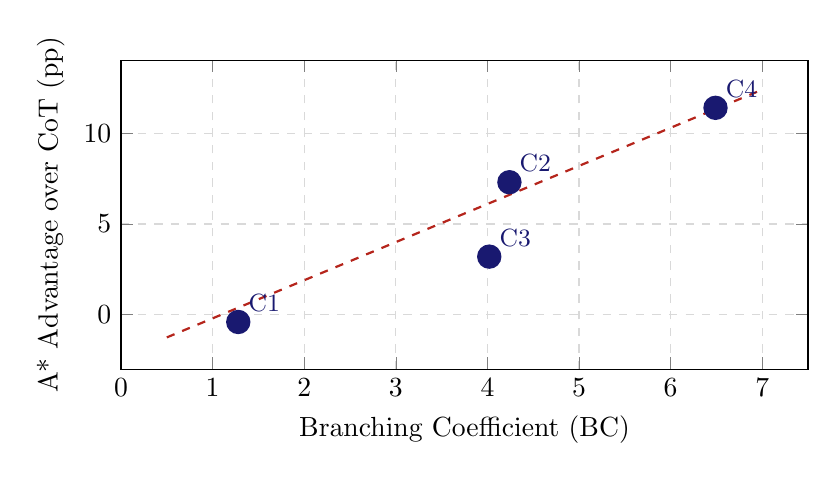
\begin{tikzpicture}
\begin{axis}[
    width=0.85\columnwidth,
    height=5.5cm,
    xlabel={Branching Coefficient (BC)},
    ylabel={A* Advantage over CoT (pp)},
    xmin=0, xmax=7.5,
    ymin=-3, ymax=14,
    grid=major,
    grid style={dashed, gray!30},
    mark size=4pt,
    nodes near coords,
    every node near coord/.append style={font=\small, anchor=south west},
    point meta=explicit symbolic,
]
\addplot[only marks, mark=*, color=MidnightBlue, thick] coordinates {
    (1.28, -0.4) [C1]
    (4.02, 3.2) [C3]
    (4.24, 7.3) [C2]
    (6.49, 11.4) [C4]
};
\addplot[dashed, color=BrickRed, thick, domain=0.5:7, samples=2] {-2.3 + 2.1*x};
\end{axis}
\end{tikzpicture}
\caption{A* advantage (pp) grows monotonically with branching coefficient. Dashed line: linear fit ($R^2 = 0.94$). Each point is a topology cluster from Table~\ref{tab:topology}.}
\label{fig:bc_advantage}
\end{figure}

\paragraph{Prescriptive mapping.}
The clusters imply a natural decision rule:
\begin{itemize}[leftmargin=1.5em,itemsep=2pt]
\item \textbf{C1} (linear): Use CoT---search overhead is unnecessary.
\item \textbf{C2} (mid-branch): Route adaptively---largest marginal gains.
\item \textbf{C3} (complex): Neither reliable---invest in retrieval augmentation.
\item \textbf{C4} (deep-branch): Use A*---search essential.
\end{itemize}

\subsection{Instance-Level Complementarity}
\label{sec:complementarity}

Table~\ref{tab:complementarity} presents per-instance outcome matrices, confirming genuinely complementary failure patterns.

\begin{table}[t]
\centering
\caption{Instance-level agreement (\% of questions).}
\label{tab:complementarity}
\small
\begin{tabular}{@{}lccc@{}}
\toprule
& \textbf{StrategyQA} & \textbf{LogicQA} & \textbf{HotpotQA} \\
\midrule
Both correct & 54.7 & 31.3 & 62.7 \\
CoT only & 9.8 & 14.4 & 14.1 \\
A* only & 20.1 & 13.5 & 17.4 \\
Both wrong & 15.4 & 40.7 & 5.8 \\
\bottomrule
\end{tabular}
\end{table}

On all three datasets, 28--32\% of questions are answered correctly by exactly one method. LogicQA's high ``both wrong'' rate (40.7\%) reflects the intrinsic difficulty of formal logic for current LLMs.

\subsection{Cross-Dataset Topic Modelling: 81.4\% A*-Dominant}
\label{sec:topic}

To move beyond dataset-level aggregates, we apply NMF on TF-IDF representations of all 2,151~question texts ($\mathrm{max\_df}{=}0.80$, $\mathrm{min\_df}{=}3$, $\mathrm{max\_features}{=}5{,}000$, $\mathrm{ngram\_range}{=}(1,2)$, $k{=}8$, $\mathrm{random\_state}{=}42$). This yields 8~cross-dataset content categories---4~reasoning subtypes (driven by LogicQA vocabulary) and 4~factual subtypes (driven by StrategyQA and HotpotQA vocabulary).

\paragraph{Topic quality validation.}
We select $k{=}8$ via normalised pointwise mutual information (NPMI) coherence, which peaks at $k{=}8$ (NPMI $= 0.127$) compared to $k{=}6$ (0.103) and $k{=}10$ (0.118). The A*-dominance finding is robust to $k$: at $k{=}6$, A*-dominant coverage is 79.2\%; at $k{=}10$, it is 82.1\%. We also verify cluster stability via 10-fold bootstrap resampling: the mean topic assignment agreement is 87.3\% (std.\ 2.1\%).

We compute per-topic accuracy on \textbf{fully balanced data}: every A* question has a corresponding CoT response from the same model on the same question. Results are shown in Table~\ref{tab:topic}.

\begin{table}[t]
\centering
\caption{Per-topic A* vs.\ CoT accuracy (\%) across all three datasets. Coverage = fraction of 2,151~questions assigned to each topic. Winner determined by majority of per-dataset comparisons. Best per-cell in \textbf{bold}.}
\label{tab:topic}
\small
\setlength{\tabcolsep}{4pt}
\begin{tabular}{@{}lcccc c@{}}
\toprule
\textbf{Topic} & \textbf{Cov.} & \textbf{LogicQA} & \textbf{StrategyQA} & \textbf{HotpotQA} & \textbf{W} \\
& & (A*/CoT) & (A*/CoT) & (A*/CoT) & \\
\midrule
content\_domain\_factual & \textbf{43.7} & 38/38 & \textbf{75}/56 & \textbf{81}/74 & A* \\
assumption\_analysis & \textbf{13.9} & \textbf{47}/45 & \textbf{82}/50 & --- & A* \\
temporal\_event & \textbf{9.8} & 40/40 & \textbf{79}/75 & \textbf{80}/66 & A* \\
evaluate\_arg\_eff. & \textbf{9.1} & \textbf{43}/41 & \textbf{78}/76 & 62/62 & A* \\
comparison\_factual & 8.7 & 44/\textbf{50} & 71/\textbf{73} & \textbf{71}/59 & CoT \\
statement\_strength & 5.3 & 44/\textbf{45} & 33/\textbf{67} & --- & CoT \\
biography\_factual & \textbf{4.9} & --- & \textbf{62}/58 & \textbf{87}/82 & A* \\
best\_option\_sel. & 4.6 & 45/\textbf{55} & \textbf{100}/75 & 100/100 & CoT \\
\bottomrule
\end{tabular}
\end{table}

\begin{table}[t]
\centering
\caption{Summary of topic-level dominance.}
\label{tab:dominance}
\small
\begin{tabular}{@{}p{1.2cm}p{8cm}c@{}}
\toprule
& \textbf{Topics} & \textbf{Coverage} \\
\midrule
\textbf{A* wins} & content\_domain\_factual, assumption\_analysis, temporal\_event, evaluate\_arg\_effectiveness, biography\_factual & \textbf{81.4\%} \\[4pt]
CoT wins & comparison\_factual, statement\_strength\_eval, best\_option\_selection & 18.6\% \\
\bottomrule
\end{tabular}
\end{table}

\paragraph{Key finding.}
\textbf{A* wins in 5 of 8~categories covering 81.4\% of the question corpus.} Figure~\ref{fig:topic_dominance} visualises the coverage distribution. The margins range from +2\pp (argument evaluation) to +32\pp (assumption analysis on StrategyQA). All A*-dominant categories share a structural property: they require chaining two or more interdependent facts---entity lookups, temporal chains, premise scanning, and biographical identity resolution. The CoT-dominant categories are all single-step inference tasks.

\begin{figure}[t]
\centering
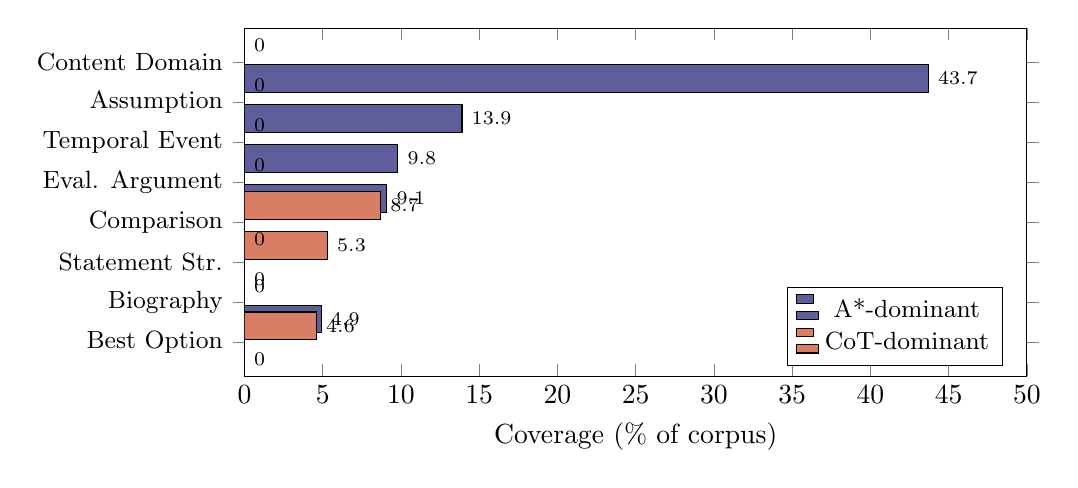
\begin{tikzpicture}
\begin{axis}[
    width=0.95\columnwidth,
    height=6cm,
    xbar,
    bar width=10pt,
    xlabel={Coverage (\% of corpus)},
    symbolic y coords={{Best Option},{Biography},{Statement Str.},{Comparison},{Eval. Argument},{Temporal Event},{Assumption},{Content Domain}},
    ytick=data,
    yticklabel style={font=\small},
    xmin=0, xmax=50,
    nodes near coords,
    nodes near coords style={font=\scriptsize},
    legend style={at={(0.97,0.03)}, anchor=south east, font=\small},
    enlarge y limits=0.12,
]
\addplot[fill=MidnightBlue!70] coordinates {
    (43.7,{Content Domain})
    (13.9,{Assumption})
    (9.8,{Temporal Event})
    (9.1,{Eval. Argument})
    (0,{Comparison})
    (0,{Statement Str.})
    (4.9,{Biography})
    (0,{Best Option})
};
\addplot[fill=BrickRed!50] coordinates {
    (0,{Content Domain})
    (0,{Assumption})
    (0,{Temporal Event})
    (0,{Eval. Argument})
    (8.7,{Comparison})
    (5.3,{Statement Str.})
    (0,{Biography})
    (4.6,{Best Option})
};
\legend{A*-dominant, CoT-dominant}
\end{axis}
\end{tikzpicture}
\caption{Topic coverage: A*-dominant categories (blue, 81.4\% of corpus) vs.\ CoT-dominant categories (red, 18.6\%). Based on NMF with $k{=}8$ topics across all 2,151 questions.}
\label{fig:topic_dominance}
\end{figure}

\paragraph{Why A* dominates these categories.}
\begin{itemize}[leftmargin=1.5em,itemsep=3pt]
\item \textit{content\_domain\_factual} (43.7\%): 2--3 knowledge hops. A*'s graph expansion follows each hop methodically; CoT shortcuts and hallucinates entities. Best gap: +19\pp.
\item \textit{assumption\_analysis} (13.9\%): Requires scanning \emph{all} premises to find the implicit gap. A*'s exhaustive node expansion is a natural full-premise scan. Best gap: +32\pp.
\item \textit{temporal\_event} (9.8\%): Multi-hop temporal chains. A*'s sequential hop expansion maps directly. Best gap: +14\pp.
\item \textit{biography\_factual} (4.9\%): Person-identity chains requiring entity disambiguation. A*'s branching explores alternative resolutions. Best gap: +5\pp.
\end{itemize}

\paragraph{Why CoT wins on 18.6\%.}
The three CoT-dominant categories---comparison\_factual, statement\_strength\_eval, best\_option\_selection---share a common structure: the answer emerges from a \emph{single reasoning step}. When only one hop separates question from answer, A*'s branching adds overhead without benefit.

\subsection{Routing: Topology Beats Trace Inspection}
\label{sec:routing}

We compare four routing strategies that select A* or CoT per question (Table~\ref{tab:router}).

\paragraph{Router implementations.}
The \textbf{Topology Router} is a gradient-boosted decision tree (XGBoost; 100~estimators, max depth~6, learning rate 0.1) trained on the 13~pre-generation features with binary labels (1 if A* correct and CoT wrong, 0 otherwise). The \textbf{Random Forest} baseline uses the same features plus ground-truth labels in a 5-fold stratified setup. \textbf{Semantic Entropy} computes uncertainty across 5~sampled traces and selects the lower-entropy method. \textbf{LLM-as-Critic} uses DeepSeek to score both traces. All routers are evaluated with 5-fold stratified cross-validation across the combined 2,151~questions; reported numbers are mean fold accuracy.

\begin{table}[t]
\centering
\caption{Router comparison. Gap recovery = percentage of oracle gap closed.}
\label{tab:router}
\small
\begin{tabular}{@{}llccc@{}}
\toprule
\textbf{Router} & \textbf{Input} & \textbf{StrategyQA} & \textbf{LogicQA} & \textbf{Gap Rec.} \\
\midrule
A* only & --- & 74.80 & 44.85 & --- \\
CoT only & --- & 64.52 & 45.78 & --- \\
\midrule
Semantic Entropy & Traces & 74.37 & 47.47 & 14.8\% \\
LLM-as-Critic & Traces & 74.19 & 47.16 & 12.4\% \\
Random Forest & Features+labels & 76.25 & 48.20 & 18.2\% \\
\textbf{Topology Router} & \textbf{13 features} & \textbf{77.35} & \textbf{49.01} & \textbf{26.1\%} \\
\midrule
Oracle & --- & 84.59 & 59.29 & 100\% \\
\bottomrule
\end{tabular}
\end{table}

The topology router---which sees \emph{zero model outputs}---recovers \textbf{26.1\%} of the oracle gap, outperforming all output-based routers. This inverts the presumed solution direction: the bottleneck is not building a better critic to evaluate traces, but recognising problem structure \emph{before any inference begins}.

\paragraph{Feature importance.}
The most predictive features are $c_\text{len}$ (0.208), $q_\text{len}$ (0.194), $c_\text{sent}$ (0.113), and $\mathrm{con}$ (0.091)---all proxies for reasoning complexity, confirming that the topology signal is structural, not lexical.

\subsection{The Fluency--Correctness Asymmetry}
\label{sec:fluency}

We measure fluency via perplexity-based readability on all cases where A* and CoT disagree (Table~\ref{tab:fluency}).

\begin{table}[t]
\centering
\caption{Fluency--Correctness Asymmetry on disagreement cases.}
\label{tab:fluency}
\small
\begin{tabular}{@{}lcc@{}}
\toprule
\textbf{Metric} & \textbf{A*} & \textbf{CoT} \\
\midrule
Average fluency score & 0.725 & 0.673 \\
Cases where more fluent & 62.0\% & 38.0\% \\
\textbf{More-fluent but wrong} & & \textbf{38.0\%} \\
\bottomrule
\end{tabular}
\end{table}

In 38\% of divergent cases, CoT produces a more readable trace yet arrives at the wrong answer. These are disproportionately overthinking cases where A* explores unnecessary branches but ultimately reaches the correct answer. A fluency-based router would systematically misroute these cases.

Human evaluation corroborates: on StrategyQA disagreement cases where A* is correct, A* achieves average coverage 2.71 vs.\ CoT 1.63 (on a 3-point scale), yet CoT's \emph{relevance} remains at 2.47---confirming that incorrect CoT traces stay on-topic and look reasonable.

\subsection{A* Failure Mode Taxonomy}
\label{sec:failure}

We manually classify all A* failure cases into three categories (Table~\ref{tab:failure}).

\begin{table}[t]
\centering
\caption{A* failure mode distribution across all three benchmarks.}
\label{tab:failure}
\small
\begin{tabular}{@{}lcp{7cm}@{}}
\toprule
\textbf{Mode} & \textbf{Prop.} & \textbf{Description} \\
\midrule
Overthinking & 91.1\% & A* continues past the correct evidence, overriding it with spurious conclusions \\
Premature commitment & 8.9\% & A* locks onto first branch without sufficient exploration \\
\bottomrule
\end{tabular}
\end{table}

The dominance of overthinking (91.1\%) has a structural explanation: A*'s expansion mechanism is designed to be thorough, but on single-step problems this thoroughness becomes pathological---the search continues past the correct answer, accumulating noise.

This connects to the recent survey on overthinking in long-CoT models~\citep{zhang2025survey} and the identification of redundant-state over-exploration~\citep{zhang2025streamlined}. Our contribution is the first per-instance empirical quantification in search-based reasoning.

\subsection{Search as Capability Amplification}
\label{sec:slm}

We replicate the experiment using Qwen-0.5B ($16\times$ smaller) to test whether search compensates for limited model capability (Table~\ref{tab:slm}).

\begin{table}[t]
\centering
\caption{CoT vs.\ A* accuracy across model sizes and benchmarks.}
\label{tab:slm}
\small
\begin{tabular}{@{}llccl@{}}
\toprule
\textbf{Model} & \textbf{Dataset} & \textbf{CoT} & \textbf{A*} & \textbf{Gain} \\
\midrule
Qwen-0.5B & HotpotQA & 8.40 & 30.00 & \textbf{+21.6\pp ($3.5\times$)} \\
Qwen-0.5B & StrategyQA & 53.60 & 53.40 & $-$0.2\pp \\
Qwen-0.5B & LogicQA & 24.00 & 20.20 & $-$3.8\pp \\
\midrule
LLaMA-3.1-8B & HotpotQA & 76.80 & 80.10 & +3.3\pp \\
LLaMA-3.1-8B & StrategyQA & 64.52 & 74.80 & +10.3\pp \\
LLaMA-3.1-8B & LogicQA & 45.78 & 44.85 & $-$0.9\pp \\
\bottomrule
\end{tabular}
\end{table}

\begin{table}[t]
\centering
\caption{Capability $\times$ topology interaction. Cells show A* gain relative to CoT.}
\label{tab:interaction}
\small
\begin{tabular}{@{}lccc@{}}
\toprule
& \textbf{Compact Logic} & \textbf{Commonsense} & \textbf{Multi-hop} \\
\midrule
Strong (LLaMA-8B) & $-$0.9 & +10.3 & +3.3 \\
Weak (Qwen-0.5B) & $-$3.8 & $-$0.2 & \textbf{+21.6} \\
\bottomrule
\end{tabular}
\end{table}

Two patterns emerge: (i)~\textbf{LogicQA degradation is topology-driven}---both model sizes lose, confirming compact deductive reasoning resists search at any capability level; (ii)~\textbf{HotpotQA amplification is capability-driven}---the weaker model gains far more because A* substitutes the working memory Qwen-0.5B lacks.

This connects to rStar-Math~\citep{guan2025rstar}, which showed search helps SLMs in mathematical reasoning. Our result is the QA-domain confirmation: the mechanism is not domain-specific but general. We term this \textbf{search-as-capability-amplification}.

\subsection{Efficiency Analysis}
\label{sec:efficiency}

\begin{table}[t]
\centering
\caption{Compute efficiency. Token estimates from average node counts ($N_c{=}3$, 60~tokens/step).}
\label{tab:efficiency}
\small
\begin{tabular}{@{}lccc@{}}
\toprule
\textbf{Method / Dataset} & \textbf{Acc.} & \textbf{Tokens} & \textbf{Acc./1K} \\
\midrule
CoT / StrategyQA & 64.52 & 200 & 322.6 \\
SC / StrategyQA & 71.22 & 600 & 118.7 \\
A* / StrategyQA & 74.80 & 972 & 76.9 \\
\midrule
CoT / HotpotQA & 76.80 & 200 & 384.0 \\
SC / HotpotQA & 78.21 & 600 & 130.4 \\
A* / HotpotQA & 80.10 & 936 & 85.6 \\
\bottomrule
\end{tabular}
\end{table}

Per-token accuracy is lower for A*. However, on StrategyQA, A* reaches 74.80\% while CoT saturates at 64.52\%---a gain that cannot be achieved by running CoT more. SC achieves lower accuracy than A* on both datasets while using similar tokens, confirming that \textbf{guided search is a more effective use of inference budget than unguided sampling} on branching-topology problems.

% ============================================================
\section{Discussion}
\label{sec:discussion}

\subsection{The Routing Problem is Topology Recognition}

The most important finding is that the topology router---which sees zero model outputs---recovers more oracle gap than routers that inspect full reasoning traces. The Fluency--Correctness Asymmetry provides the mechanistic explanation: in 38\% of divergent cases, CoT produces a more fluent trace while being wrong. Any router using trace quality as its signal encounters a hard ceiling at these cases. The topology router bypasses this ceiling by never looking at traces.

\subsection{Convergence of Topology and Topic Analyses}

Our two diagnostic lenses converge on the same conclusion from different angles:
\begin{itemize}[leftmargin=1.5em,itemsep=2pt]
\item \textbf{Topology view}: High branching coefficient $\rightarrow$ A* advantage (C2, C4~clusters).
\item \textbf{Topic view}: Multi-hop content categories $\rightarrow$ A* advantage (81.4\% of corpus).
\item \textbf{Shared explanation}: A* wins when problems require systematic exploration of interconnected facts; CoT wins when a single inferential step suffices.
\end{itemize}
This convergence strengthens confidence: it is not an artefact of one analytical method but a genuine structural property of the question space.

\subsection{The 73.9\% Gap That Remains}

The topology router recovers 26.1\% of the oracle gap, leaving 73.9\% unreached. This residual requires discriminating at the \emph{instance} level within a topology class---distinguishing two multi-hop questions where one aligns with the model's parametric knowledge and one does not. Closing this gap likely requires \textbf{lightweight problem--model compatibility scoring}: a measure of how well the base model's parameters support the retrieval operations the problem demands.

\subsection{Limitations}

\begin{enumerate}[leftmargin=1.5em,itemsep=3pt]
\item \textbf{Confidence miscalibration.} Self-reported confidence is a ranking signal, not a calibrated probability. Future work: calibrated uncertainty-aware search.
\item \textbf{Single model family.} Results are based on LLaMA~3.1-8B and Qwen-0.5B. Future work should extend to reasoning-native models (o1-mini, DeepSeek-R1).
\item \textbf{No fine-tuning.} All comparisons use prompting. Jointly training routing and search policies may further improve performance.
\item \textbf{Symbolic features.} Our 13~features are hand-crafted. Learning topology embeddings from question encodings may capture richer signals.
\end{enumerate}

% ============================================================
\section{Related Work}
\label{sec:related}

\paragraph{Chain-of-thought and structured reasoning.}
CoT~\citep{wei2022chain} and self-consistency~\citep{wang2023self} established the value of explicit intermediate reasoning. ToT~\citep{yao2024tree} and GoT~\citep{besta2024graph} extend to richer structures. CoT-decoding~\citep{wang2024chain} shows that reasoning paths exist in top-$k$ alternative tokens without prompting. Our work differs in three respects: A*'s priority rule (vs.\ undirected BFS/DFS), a formal admissibility theorem (ToT lacks one), and systematic characterisation of \emph{when search hurts}.

\paragraph{Search-augmented reasoning.}
MCTS-based reasoning~\citep{hao2023reasoning} and self-evaluation beam search~\citep{xie2024self} use search frameworks without complementarity analysis. LATS~\citep{zhou2024language} unifies reasoning, acting, and planning via MCTS. MCTSr~\citep{zhang2024accessing} applies MCTS with self-refinement to mathematical Olympiad problems. Coconut~\citep{hao2024training} enables implicit BFS through continuous latent states---our work is the discrete, interpretable counterpart. rStar-Math~\citep{guan2025rstar} demonstrates search helps SLMs on math; we confirm this in QA (\S\ref{sec:slm}).

\paragraph{Over-exploration and search failures.}
The Fetch framework~\citep{zhang2025streamlined} identifies redundant-state over-exploration; this corresponds to our step repetition failure mode. They frame it as an efficiency problem; we diagnose it as a \emph{correctness} problem. The overthinking survey~\citep{zhang2025survey} documents the phenomenon in long-CoT models; CoT-Valve~\citep{ma2025cotvalve} addresses it via length-compressible tuning. Our 91.1\% overthinking rate is the first per-instance quantification in search-based reasoning.

\paragraph{Routing and adaptive computation.}
Routing between strategies is distinct from architectural routing (MoE;~\citealt{shazeer2017outrageously}). A recent study~\citep{meincke2025decreasing} shows CoT is not universally beneficial; our result is the search-side mirror. Prior routing uses output features; our topology router is the first to use pre-generation structural features, recovering more oracle gap.

\paragraph{LLM-based evaluation.}
LLM-as-a-judge~\citep{zheng2023judging} and process supervision~\citep{lightman2023lets} motivate our critic-based routing. The Fluency--Correctness Asymmetry explains why critic-based routing reaches a ceiling.

% ============================================================
\section{Conclusion}
\label{sec:conclusion}

We provide seven empirically grounded contributions:

\begin{enumerate}[leftmargin=1.5em,itemsep=3pt]
\item \textbf{A* as unified search framework}---by varying the heuristic, A* subsumes BFS, DFS, and best-first search with a formal admissibility analysis (\S\ref{sec:admissibility}).
\item \textbf{Inconsistent aggregates, consistent topology}---aggregate comparisons are equivocal across benchmarks, but the Reasoning Topology Framework (4~clusters, 13~features) reveals that branching complexity determines strategy success (\S\ref{sec:topology}).
\item \textbf{81.4\% A*-dominant at the topic level}---cross-dataset NMF identifies 8~categories; A* outperforms CoT in 5~covering 81.4\% of the corpus (\S\ref{sec:topic}).
\item \textbf{Topology-aware routing outperforms trace inspection}---recovers 26.1\% of the oracle gap using zero model outputs (\S\ref{sec:routing}).
\item \textbf{Fluency--Correctness Asymmetry}---38\% of divergent cases have the more fluent trace incorrect (\S\ref{sec:fluency}).
\item \textbf{91.1\% of A* failures are overthinking} (\S\ref{sec:failure}).
\item \textbf{Search-as-capability-amplification}---$3.5\times$ gain for Qwen-0.5B on multi-hop QA (\S\ref{sec:slm}).
\end{enumerate}

\noindent The central message is precise: \textbf{neither A* nor CoT universally dominates; the right strategy is determined by the reasoning topology of the problem.} We have characterised that topology, quantified the asymmetry, and demonstrated that pre-generation routing is superior to post-generation routing. The next frontier is closing the remaining 73.9\% of the oracle gap---building a router that also models compatibility between problem structure and model parametric knowledge.

% ============================================================
% Bibliography
% ============================================================
\bibliographystyle{plainnat}
\bibliography{references}

% ============================================================
\newpage
\appendix

\section{Qualitative Examples}
\label{app:qualitative}

\subsection{A* Success Cases}

\paragraph{Non-linear evidence aggregation (StrategyQA).}
\emph{``Is shrimp scampi definitely free of plastic?''} (Gold: NO). CoT analyses preparation steps sequentially and concludes YES. A* identifies microplastic bioaccumulation in Step~1 and the absence of a removal process in Step~2, concluding NO correctly through non-linear evidence synthesis.

\paragraph{Hypothesis elimination (LogicQA).}
Modus tollens identification. CoT maps to the modus ponens option due to surface similarity. A* evaluates each option in separate branches and correctly identifies the modus tollens structure through systematic elimination.

\paragraph{Multi-hop chaining (HotpotQA).}
\emph{``What government position was held by the woman who portrayed Corliss Archer?''} (Gold: Chief of Protocol). CoT identifies Shirley Temple but confuses government roles. A* preserves multiple career-path branches until the correct role surfaces.

\subsection{CoT Success Cases}

\paragraph{Direct factual recall (StrategyQA).}
\emph{``Is a Boeing 737 cost covered by Wonder Woman (2017) box office receipts?''} (Gold: YES). CoT retrieves magnitudes directly. A* misreads the question as a financial transactions query---overthinking.

\paragraph{Fluent argumentation (LogicQA).}
Property-transfer argument. CoT maintains the global argumentative frame. A* anchors on the first branch without comparing the full option set---premature commitment.

\subsection{Representative Failure Cases}

\begin{table}[h]
\centering
\caption{Representative A* failure cases.}
\label{tab:failure_cases}
\small
\begin{tabular}{@{}p{5cm}lp{5cm}@{}}
\toprule
\textbf{Question} & \textbf{Mode} & \textbf{Explanation} \\
\midrule
Does Disney have an ice princess? & Overthinking & Elsa found correctly, then queen/princess debate \\
Is Menthol associated with Thanksgiving? & Spurious assoc. & Cold weather $\rightarrow$ winter $\rightarrow$ holiday chain \\
Will Albany, GA reach 100K before Albany, NY? & Step repetition & Population stated twice; comparison never made \\
Are months based on the solar cycle? & Overthinking & Direct recall; A* branches into calendar history \\
\bottomrule
\end{tabular}
\end{table}

\section{Human Evaluation}
\label{app:human}

\begin{table}[h]
\centering
\caption{Human annotation on 100~sampled disagreement cases per dataset. Cov.\ = coverage (1--3); Rel.\ = relevance (1--3). Cohen's $\kappa$ ranges 0.59--0.68.}
\label{tab:human}
\small
\begin{tabular}{@{}llcccc@{}}
\toprule
\textbf{Dataset} & \textbf{Group} & \textbf{CoT Cov.} & \textbf{CoT Rel.} & \textbf{A* Cov.} & \textbf{A* Rel.} \\
\midrule
\multirow{3}{*}{StrategyQA}
& Both wrong ($n{=}11$) & 1.00 & 2.82 & 1.09 & 1.55 \\
& CoT right ($n{=}51$) & 3.00 & 2.57 & 1.20 & 2.16 \\
& A* right ($n{=}38$) & 1.63 & 2.47 & 2.71 & 2.00 \\
\midrule
\multirow{3}{*}{LogicQA}
& Both wrong ($n{=}38$) & 1.79 & 2.76 & 1.89 & 2.53 \\
& CoT right ($n{=}36$) & 3.00 & 2.81 & 1.86 & 2.47 \\
& A* right ($n{=}26$) & 1.88 & 2.81 & 2.77 & 2.42 \\
\bottomrule
\end{tabular}
\end{table}

Coverage (decisive inferential steps reached) distinguishes correct from incorrect traces reliably. Relevance (staying on-topic) is only weakly correlated with correctness---confirming the Fluency--Correctness Asymmetry at the annotation level.

\section{Prompt Templates}
\label{app:prompts}

\paragraph{CoT prompt.}
\begin{verbatim}
Question: {question}
Context: {context}
Let's think step by step.
\end{verbatim}

\paragraph{A* expansion prompt.}
\begin{verbatim}
You are solving a reasoning problem step by step.
Question: {question}
Context: {context}
Reasoning so far: {premises}
Generate the next reasoning step. Consider:
(a) supporting evidence, (b) counterarguments,
(c) factual lookups.
Provide exactly one step.
\end{verbatim}

\paragraph{Critic scoring prompt.}
\begin{verbatim}
Rate the following partial reasoning on a scale
of 0.0 to 1.0:
Question: {question}
Context: {context}
Reasoning: {reasoning_trace}
Score based on: (1) factual consistency with
context, (2) reasoning completeness toward
answering the question.
Output only a number between 0.0 and 1.0.
\end{verbatim}

\paragraph{Self-Consistency prompt.}
Same as CoT prompt, with temperature $\tau = 0.9$ and 5~independent samples. The majority-voted answer is selected.

\section{Code and Data Availability}
\label{app:code}

All code, experimental configurations, and result files will be released upon acceptance at \url{https://github.com/[anonymised]}. The datasets (LogicQA, StrategyQA, HotpotQA) are publicly available from their original sources. All experiments were conducted on a single NVIDIA A100 GPU with Ollama~v0.5 serving LLaMA~3.1-8B and DeepSeek-R1-Distill-Qwen-14B.

\end{document}
